\chapter{Time and Global States}
\begin{multicols*}{2}

\noindent Although one of the property of distributed system is no globally shared clock, many distributed applications still depend on timing.

\section{Synchronizing Physical Clock}

\noindent Computers have their own physical clocks that deviate from one another. Universal Coordinated Time (UTC) is commonly used reference clock.\\

\noindent \emph{Clock drift}: clock count time at different rates.\\

\noindent \emph{Drift rate}: the change in offset between a clock and a perfect reference clock per unit of time measured by the reference clock.

\subsection{Cristian's Method}

\noindent The algorithm:

\begin{enumerate}
  \item $A$ requests the time of $B$
  \item $B$ replies with the time value $t$
  \item $A$ records the total RTT, $T_{\text{round}}=t_2 - t_1$
  \item $A$ sets its clock to $t + T_{\text{round}} / 2$
\end{enumerate}

\noindent To calculate the accuracy of Cristian's Method, we need to consider 2 cases:
\begin{enumerate}
  \item When the transmission time of reply message approaches $0$, $B$'s clock reading is $t$.
  \item When the transmission time of reply message approaches $T_{\text{round}}$, $B$'s clock reading is $t+ T_{\text{round}}$.
\end{enumerate}

\noindent When $A$ receives the reply, the time reading on $B$ should be in $[t,t+ T_{\text{round}}]$. $A$ is accurate within bound $T_{\text{round}} / 2$

\subsection{Berkeley Algorithm}

\noindent The algorithm:
\begin{enumerate}
  \item Master periodically polls slaves
  \item Slaves send their clock readings back
  \item Master evaluates the local times of slaves by observing the RTT
  \item Master averages the values obtained and its own clock reading
  \item Master sends the amount of adjustment to each slave
\end{enumerate}

\noindent We use average clock reading because it cancels out individual clocks' tendencies to run fast or slow.

\subsection{Network Time Protocol}

\noindent Cristian's method and Berkeley algorithm use centralized design. Network Time Protocol (NTP) is used to distribute time information over the Internet. \\

\noindent NTP has a network of servers structured hierarchically into a synchronization subnet. This setup is fault-tolerance because servers can reconfigure themselves if someone becomes unreachable.

\subsubsection{Analysis of Accuracy}
\begin{center}
\begin{tikzpicture}[>=stealth',thick,
commentl/.style={text width=0.7cm, align=right},
commentr/.style={commentl, align=left},]
\node[] (init) {Server B};
\node[right=1cm of init] (recv) {Server A};

\draw[->] ([yshift=-.5cm]init.south) coordinate (send1) -- ([yshift=-.7cm]send1-|recv) coordinate (send1done) node[pos=.3, above, sloped] {};

\draw[->] ([yshift=-.3cm]send1done) coordinate (reply1) -- ([yshift=-.7cm]reply1-|init) coordinate (reply1done) node[pos=.3, above, sloped] {m};

\draw[->] ([yshift=-1cm]reply1done) coordinate (send2) -- ([yshift=-.7cm]send2-|recv) coordinate (send2done) node[pos=.3, above, sloped] {m'};

\draw[->] ([yshift=-.3cm]send2done) coordinate (reply2) -- ([yshift=-.7cm]reply2-|init) coordinate (reply2done) node[pos=.3, above, sloped] {};

\draw[thick, shorten >=-1cm] (init) -- (init|-reply2);
\draw[thick, shorten >=-1cm] (recv) -- (recv|-reply2);

\node[commentr, right =1mm of reply1] {$T_{i-3}$};
\node[left = 1mm of reply1done.west, commentl]{$T_{i-2}$};
\node[left = 1mm of send2.west, commentl]{$T_{i-1}$};
\node[commentr, right =1mm of send2done] {$T_{i}$};
\end{tikzpicture}
\end{center}

\noindent Time between sending of $m$ and receipt of $m'$ is $$T_i - T_{i-3}$$
\noindent Time between receipt of $m$ and sending of $m'$ is $$T_{i-1} - T_{i-2}$$
\noindent The total transmission time of $m$ and $m'$ is $$(T_i - T_{i-3}) - (T_{i-1} - T_{i-2})$$
\noindent The transmission time of $m'$ is $$[0,(T_i - T_{i-3}) - (T_{i-1} - T_{i-2})]$$
\noindent If transmission time of $m'$ approaches $0$, when A receives $m'$ B clock reading is $$T_{i-1}$$
\noindent If transmission time of $m'$ approaches $(T_i - T_{i-3}) - (T_{i-1} - T_{i-2})$, when A receives $m'$ B clock reading is $$T_{i-1} + (T_i - T_{i-3}) - (T_{i-1} - T_{i-2}) = T_i - T_{i-3} + T_{i-2}$$
\noindent If A want to synchronize with B as accurately as possible, A should set its clock to $$\frac{1}{2}(T_{i-1} + (T_i - T_{i-3} + T_{i-2})$$

\noindent The accuracy is $$\pm \frac{1}{2}(T_{i-1} - (T_i - T_{i-3} + T_{i-2})$$

\section{Causal Ordering and Logical Clocks}

\noindent We refer the state of process $p_i$ and as $s_i$, and there are $i=1\ldots N$ number of processes.\\

\noindent Process takes a series of actions, i.e. sending a message, receiving a message, or transforms the state of the process.\\

\noindent An event is the occurrence of a single action.

\subsection{Causal Ordering}

\noindent Events can be ordered based on cause-and-effect. Event within a single process $p_i$ can be placed in a unique total ordering. The event of sending the message occurs before the event of receiving the message.

\begin{center}
\begin{tikzpicture}[>=stealth',thick,
roundnode/.style={circle, draw=black, thick, minimum size=0.7cm},
]
\node[] (p1) {$p_1$};
\node[below=1cm of p1] (p2) {$p_2$};
\node[below=1cm of p2] (p3) {$p_3$};

\node[roundnode](a)[right = 1mm of p1.east]{a};
\node[roundnode](b)[right = 12mm of a.east]{b};

\node[roundnode](c)[right = 25mm of p2.east]{c};
\node[roundnode](d)[right = 12mm of c.east]{d};

\node[roundnode](e)[right = 12mm of p3.east]{e};
\node[roundnode](f)[right = 50mm of p3.east]{f};

\node[right = 60mm of p1](d1){};
\node[right = 60mm of p2](d2){};
\node[right = 60mm of p3](d3){};

\draw[-] (a) -- (b) node [pos=0.5, above, align=center] {$a\rightarrow b$};
\draw[->] (b) -- (c) node [pos=0.3, right, align=center] {$b\rightarrow c$};
\draw[-] (c) -- (d) node [pos=0.5, above, align=center] {$c\rightarrow d$};
\draw[->] (d) -- (f) node [pos=0.3, right, align=center] {$d\rightarrow f$};
\draw[-] (e) -- (f) node [pos=0.5, above, align=center] {$e\rightarrow f$};
% Dummy
\draw[-] (b) -- (d1);
\draw[-] (p2) -- (c);
\draw[-] (d) -- (d2);
\draw[-] (p3) -- (e);
\draw[-] (f) -- (d3);

\end{tikzpicture}
\end{center}

\noindent From the figure above, we can deduce that $a$ happens before $f$, $a\rightarrow f$, and $a$ is parallel to $e$, $a\|e$

\subsection{Lamport's Logical Clocks}

\noindent Logical clock is a monotonically increasing software counter whose value bears no particular relationship with real time.

\begin{center}
\begin{tikzpicture}[>=stealth',thick,
roundnode/.style={circle, draw=black, thick, minimum size=0.7cm},
]
\node[] (p1) {$p_1$};
\node[below=1cm of p1] (p2) {$p_2$};
\node[below=1cm of p2] (p3) {$p_3$};

\node[roundnode](a)[right = 1mm of p1.east]{a};
\node[roundnode](b)[right = 12mm of a.east]{b};

\node[roundnode](c)[right = 30mm of p2.east]{c};
\node[roundnode](d)[right = 12mm of c.east]{d};

\node[roundnode](e)[right = 12mm of p3.east]{e};
\node[roundnode](f)[right = 60mm of p3.east]{f};

\node[right = 80mm of p1](d1){};
\node[right = 80mm of p2](d2){};
\node[right = 80mm of p3](d3){};

\draw[-] (a) -- (b) node [pos=0.5, below = 5mm, align=center] {$a\rightarrow b\ (1<2)$};
\draw[->] (b) -- (c) node [pos=0, right = 3mm, align=center] {$b\rightarrow c\ (2<3)$};
\draw[-] (c) -- (d) node [pos=0.5, below = 5mm, align=center] {$c\rightarrow d\ (3<4)$};
\draw[->] (d) -- (f) node [pos=0, right = 3mm, align=center] {$d\rightarrow f\ (4<5)$};
\draw[-] (e) -- (f) node [pos=0.5, below, align=center] {$e\rightarrow f\ (1<5)$};

% Dummy
\draw[-] (b) -- (d1);
\draw[-] (p2) -- (c);
\draw[-] (d) -- (d2);
\draw[-] (p3) -- (e);
\draw[-] (f) -- (d3);

% Label
\node[above=1mm of a](labela){1};
\node[above=1mm of b](labelb){2};
\node[above=1mm of c](labelc){3};
\node[above=1mm of d](labeld){4};
\node[above=1mm of e](labele){1};
\node[above=1mm of f](labelf){5};

\end{tikzpicture}
\end{center}

\noindent From the diagram above, since $a\rightarrow f$, so $L(a)<L(e')$. This is always true, but the converse is not. Specifically, if $L(e)<L(e')$, we cannot infer that $e\rightarrow e'$.

\subsection{Vector Clocks}

\noindent A vector clock for $N$ processes is an array of $N$ integers. Each process has its own vector clock.

\begin{center}
\begin{tikzpicture}[>=stealth',thick,
roundnode/.style={circle, draw=black, thick, minimum size=0.7cm},
]
\node[] (p1) {$p_1$};
\node[below=1cm of p1] (p2) {$p_2$};
\node[below=1cm of p2] (p3) {$p_3$};

\node[roundnode](a)[right = 1mm of p1.east]{a};
\node[roundnode](b)[right = 12mm of a.east]{b};

\node[roundnode](c)[right = 35mm of p2.east]{c};
\node[roundnode](d)[right = 12mm of c.east]{d};

\node[roundnode](e)[right = 12mm of p3.east]{e};
\node[roundnode](f)[right = 70mm of p3.east]{f};

\node[right = 80mm of p1](d1){};
\node[right = 80mm of p2](d2){};
\node[right = 80mm of p3](d3){};

\draw[-] (a) -- (b) node [pos=0.5, below = 5mm, align=center] {$a\rightarrow b$};
\draw[->] (b) -- (c) node [pos=0, right = 3mm, align=center] {$b\rightarrow c$};
\draw[-] (c) -- (d) node [pos=0.5, below = 5mm, align=center] {$c\rightarrow d$};
\draw[->] (d) -- (f) node [pos=0, right = 3mm, align=center] {$d\rightarrow f$};
\draw[-] (e) -- (f) node [pos=0.5, below, align=center] {$e\rightarrow f$};

% Dummy
\draw[-] (b) -- (d1);
\draw[-] (p2) -- (c);
\draw[-] (d) -- (d2);
\draw[-] (p3) -- (e);
\draw[-] (f) -- (d3);

% Label
\node[above=1mm of a](labela){(1,0,0)};
\node[above=1mm of b](labelb){(2,0,0)};
\node[above=1mm of c](labelc){(2,1,0)};
\node[above=1mm of d](labeld){(2,2,0)};
\node[above=1mm of e](labele){(0,0,1)};
\node[above=1mm of f](labelf){(2,2,2)};

\end{tikzpicture}
\end{center}

\noindent If $e\rightarrow e'$, then $V(e)\rightarrow V(e')$.

\noindent If $V(e)\rightarrow V(e')$, then $e\rightarrow e'$.

\noindent If $e\|e'$, then neither $V(e)\le V(e')$ nor $V(e')\le V(e)$

\section{Global States}

\noindent In many situations, we need to find out whether a particular property is true when a distributed system executes. We want to assemble a meaningful global state from local states recorded by different process at different real times.\\

\noindent The state of process $p_i$ is the state immediately after its $k$-th event occurs. Global state is a set of states of all processes.

\subsection{Consistent Cut} \label{section:consistent-cut}

\noindent A consistent cut is a cut $C$, such that for all events $\forall e\in C$, $\exists f \in C, f\rightarrow e$. Otherwise, the cut is unconsistent.

\tiny
\begin{center}
\begin{tikzpicture}[>=stealth',thick,
roundnode/.style={circle, draw=black, thick, minimum size=0.3cm},
]

\node[] (p1) {$p_1$};
\node[below=1cm of p1] (p2) {$p_2$};

\node[roundnode](e11)[right = 1mm of p1.east]{$e_1^1$};
\node[roundnode](e12)[right = 5mm of e11.east]{$e_1^2$};
\node[roundnode](e13)[right = 5mm of e12.east]{$e_1^3$};
\node[roundnode](e14)[right = 43mm of e13.east]{$e_1^4$};

\node[roundnode](e21)[right = 37mm of p2.east]{$e_2^1$};
\node[roundnode](e22)[right = 5mm of e21.east]{$e_2^2$};
\node[roundnode](e23)[right = 5mm of e22.east]{$e_2^3$};

\node[right = 83mm of p1](d1){};
\node[right = 83mm of p2](d2){};

\draw[-] (e11) -- (e12);
\draw[-] (e12) -- (e13);
\draw[-] (e13) -- (e14);

\draw[->] (e12) -- (e21) node [pos=0.5, right = 3mm, align=center] {$m_1$};
\draw[-] (e21) -- (e22);
\draw[-] (e22) -- (e23);
\draw[->] (e23) -- (e14) node [pos=0.3, right = 3mm, align=center] {$m_2$};

% Dummy
\draw[-] (p2) -- (e21);
\draw[-] (e14) -- (d1);
\draw[-] (e23) -- (d2);

\draw[dashed]
  ([yshift=10pt]$ (e13)!0.5!(e14) $ ) --
  ([yshift=-25pt]$ (e13)!0.5!(p2) $ ) node [below = 1mm] {consistent};

\end{tikzpicture}
\end{center}
\normalsize

\subsection{Recording a Snapshot}

\noindent To record a snapshot, we need to record the states of all processes and the state of communication channels.

\subsubsection{Chandy and Lamport Algorithm}

\noindent The algorithm uses a marker messages to prompt the receiver to save its own local state and determine which messages to include in the channel state.

\noindent The algorithm:

\begin{itemize}
  \item Any process may initiate a snapshot recording at any time
  \item Each non-initiating process records its process state on receiving the first marker message
  \item If $p_j$ is the initiating process, $p_j$ initiates the messages arriving on channel $c_{i\rightarrow j}$ between $p_j$ initiates the snapshot recording and receives the marker message from $p_i$
  \item If $p_j$ is non-initiating process and $c_{i\rightarrow j}$ is the channel through which $p_j$ receives its first marker message, $c_{i\rightarrow j}$ state is recorded as an empty set
  \item If $p_j$ is non-initiating process and $c_{i\rightarrow j}$ is not the channel through which $p_j$ receives its first marker message, $p_j$ records the message arriving on channel $c_{i\rightarrow j}$ between $p_j$ receives the first marker message and the marker message from $p_i$
  \item Each process completes all recording activities when it has received a marker message from all other processes. Then, it may send the recorded states (local process state + channel states) to the initiating process.
\end{itemize}

\section{Distributed Debugging}

\noindent We want to establish what occurred during the execution of a distributed system and to check whether they are correct.

\subsection{Lattice of Consistent Global States}

\noindent Referring to the figure in section \ref{section:consistent-cut}, we will get the following lattice of consistent global states. The lattice is constructed by listing all consistent global states starting from the initial state and advance the global state by one event at a time.

\begin{center}
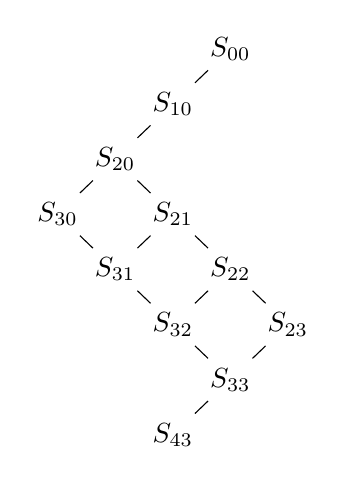
\begin{tikzpicture}[
recnode/.style={rectangle, draw=white, thin},
level distance=0.7cm,
level 1/.style={sibling distance=0.7cm},
level 2/.style={sibling distance=0.7cm},
level 3/.style={sibling distance=0.7cm},
level 4/.style={sibling distance=0.7cm},
level 5/.style={sibling distance=0.7cm},
level 6/.style={sibling distance=0.7cm},
level 7/.style={sibling distance=0.7cm},
level 8/.style={sibling distance=0.7cm},
]
%Nodes
\node[recnode,draw](s00){$S_{00}$}
  child[left] {node[recnode,draw](s10){$S_{10}$} edge from parent[-]
    child[left] {node[recnode,draw](s20){$S_{20}$} edge from parent[-]
      child[left] {node[recnode,draw](s30){$S_{30}$} edge from parent[-]}
      child[right] {node[recnode,draw](s21){$S_{21}$} edge from parent[-]
        child[left] {node[recnode,draw](s31){$S_{31}$} edge from parent[-]}
        child[right] {node[recnode,draw](s22){$S_{22}$} edge from parent[-]
          child[left] {node[recnode,draw](s32){$S_{32}$} edge from parent[-]}
          child[right] {node[recnode,draw](s23){$S_{23}$} edge from parent[-]
            child[left] {node[recnode,draw](s33){$S_{33}$} edge from parent[-]
              child[left] {node[recnode,draw](s43){$S_{43}$} edge from parent[-]}
              child[missing] {node[recnode,draw](d){} edge from parent[-]}
            }
            child[missing] {node[recnode,draw](d){} edge from parent[-]}
          }
        }
      }
    }
    child[missing] {node[recnode,draw](d){} edge from parent[-]}
  }
  child[missing] {node[recnode,draw](d){} edge from parent[-]}
;

\draw (s31) -- (s30);
\draw (s32) -- (s31);
\draw (s33) -- (s32);
\end{tikzpicture}
\end{center}

\noindent Each path from top-level state to the bottom level state in the lattice represents an ordering of all events that are consistent with causal ordering. Without global time, we cannot tell which one is the actual execution of the system among all possible executions.\\

\noindent In general, $<s_1^{c_i}, s_2^{c_j},\ldots,s_N^{c_N}>$ is a consistent global state if $V(e_i^{c_i})[i] \ge V(e_j^{c_j})[i]$ for any $i$ and $j$. \\

\noindent If there are only two processes, $S_{ij} = <s_1^{i}, s_2^{j}>$ is a consistent global state if $V(e_1^{i})[1] \ge V(e_2^{j})[1]$ and $V(e_2^{j}[2]) \ge V(e_1^{i})[2]$\\

\noindent To check whether a constraint is broken during execution, we need to evaluate whether each global state satisfies the constraint:
\begin{itemize}
  \item If all states satisfy the constraint, the constraint cannot be broken in the execution
  \item If there exists a state not satisfying the constraint, the constraint is possibly broken in the execution
  \item If every path from top to bottom passes through at least one state that does not satisfy the constraint, the constraint must be broken in the execution
\end{itemize}

\end{multicols*}
